\documentclass[tikz,border=5pt]{standalone}
\usepackage{pgfplots}
\pgfplotsset{compat=1.18}

\definecolor{corba}{HTML}{365FB3}
\definecolor{punt}{HTML}{B91C1C}
\definecolor{guia}{HTML}{6B7280}

\begin{document}
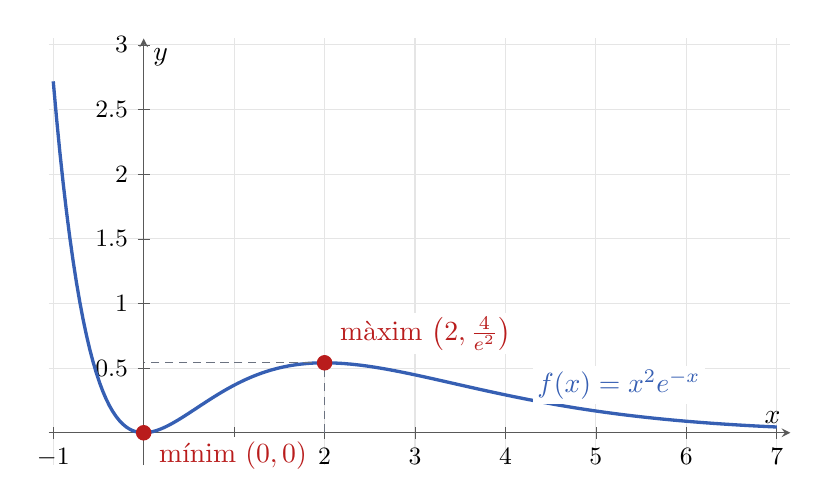
\begin{tikzpicture}
  \begin{axis}[
    width=11cm,
    height=7cm,
    axis lines=middle,
    xmin=-1.05,
    xmax=7.15,
    ymin=-0.25,
    ymax=3.05,
    xlabel={$x$},
    ylabel={$y$},
    xtick={-1,0,1,2,3,4,5,6,7},
    ytick={0.5,1,1.5,2,2.5,3},
    grid=major,
    grid style={black!10},
    axis line style={black!65},
    tick style={black!65},
    tick label style={font=\small},
    clip=false,
  ]
    \addplot[corba, very thick, domain=-1:7, samples=220]
      {x^2*exp(-x)};

    \draw[guia, densely dashed]
      (axis cs:2,0) -- (axis cs:2,{4/exp(2)}) -- (axis cs:0,{4/exp(2)});

    \addplot[only marks, mark=*, mark size=2.6pt, punt]
      coordinates {(0,0) (2,{4/exp(2)})};

    \node[anchor=north west, text=punt, fill=white, inner sep=1.5pt]
      at (axis cs:0.12,-0.03) {mínim $(0,0)$};
    \node[anchor=south west, text=punt, fill=white, inner sep=1.5pt]
      at (axis cs:2.12,{4/exp(2)+0.06}) {màxim $\left(2,\frac{4}{e^2}\right)$};
    \node[anchor=south west, text=corba, fill=white, inner sep=1.5pt]
      at (axis cs:4.3,0.22) {$f(x)=x^2e^{-x}$};
  \end{axis}
\end{tikzpicture}
\end{document}
